% chap4.tex (Definitions and Theorem)

\chapter{Model, Dataset, and Final Pipeline Description}
\section{Layer Descriptions}
\subsection{Embedding Layer}
An \textbf{embedding layer} maps an word index, or integer, into its corresponding embedding.
This layer is usually the first layer in a neural network that processes input such as text.
Given input text $s$, this layer receives as input a sequence of word indexes $BoW(\bm{s})=$ $\bm{x} = x_1,...,x_k$
and maps each word into an embedding.
Thus, for an input text $\bm{s}$, we transform it into a sequence of integers $\bm{x}$, and from there into $\mathbf{E} \in \mathbb{R}^{n \times d}$, where $d$ is
the embedding size. These embeddings are further fine-tuned during training. Because of the large number of
parameters in this layer (number of words allowed times embedding size), it is usually a good idea to
use $L_2$ regularization or dropout in order to avoid or mitigate overfitting.

\begin{figure}[H]
\caption{Visualization of an embedding layer. Word indexes are mapped to word embeddings. This
layer outputs a matrix comprised of stacked embeddings, one for each index.}
\centering
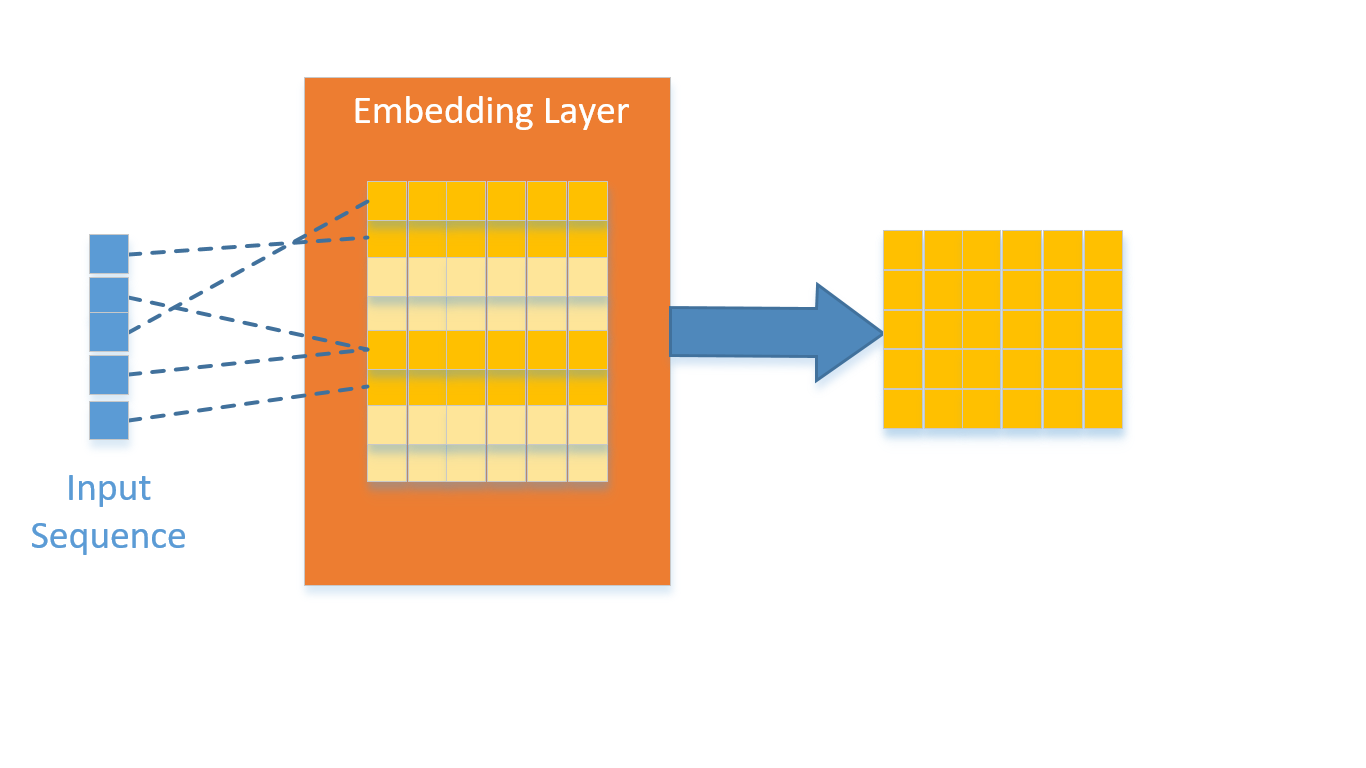
\includegraphics[width=0.5\textwidth]{EmbeddingLayer.png}
\end{figure}

\subsection{Feature Maps: Convolution + Pooling}

We refer to a pair of convolutional layer followed by a pooling layer as a feature map.

\subsection{Gated Recurrent Unit Layer}
A Gated Recurrent Unit layer is a type of recurrent layer designed to combat the vanishing gradient
problem [CITE]. It is a simplified version of the LSTM layer, and in practice it performs comparably.
Because of this, we choose this particular layer for a recurrent layer.

\subsection{Dense Layer}
The last layer in our model is the classical \textbf{dense}, or fully connected layer.
The number of units in this layer is equal to the number of classes in our dataset.
Each unit $h_i$ is a linear combination of the previous layer's output with the unit's
corresponding set of weights. The \textbf{softmax} activation function is then applied to
the units, to finally output class probabilities.


\section{Model Description}

A standard architecture for convolutional neural networks for text sequence classification is the one proposed by
[CITE YOON 2014]. This model has an embedding layer followed by a feature map and a dense layer with a softmax activation
to output class probabilities.

Another popular neural model for text classification is the recurrent neural network, where each. This model is
essentially an embedding layer followed by a recurrent layer e.g. LSTM or GRU, then a dense layer to output probabilities.
Our model is a mixture of these two standards: after the embedding layer, we add a feature map to learn the spatial
structure of the data, then we add a GRU layer. This design choice was made due to the fact that a recurrent layer
always led to better model performance, while the convolutional/pooling operations led to a huge data dimensionality reduction
and thus much faster training times. The two types of layers, combined, performed the best.


\begin{figure}[h]
\caption{Model Architecture: embedding layer, followed by two feature maps, and a recurrent layer. At the end, we have
a fully connected layer with a softmax activation, which will output class probabilities.}
\centering
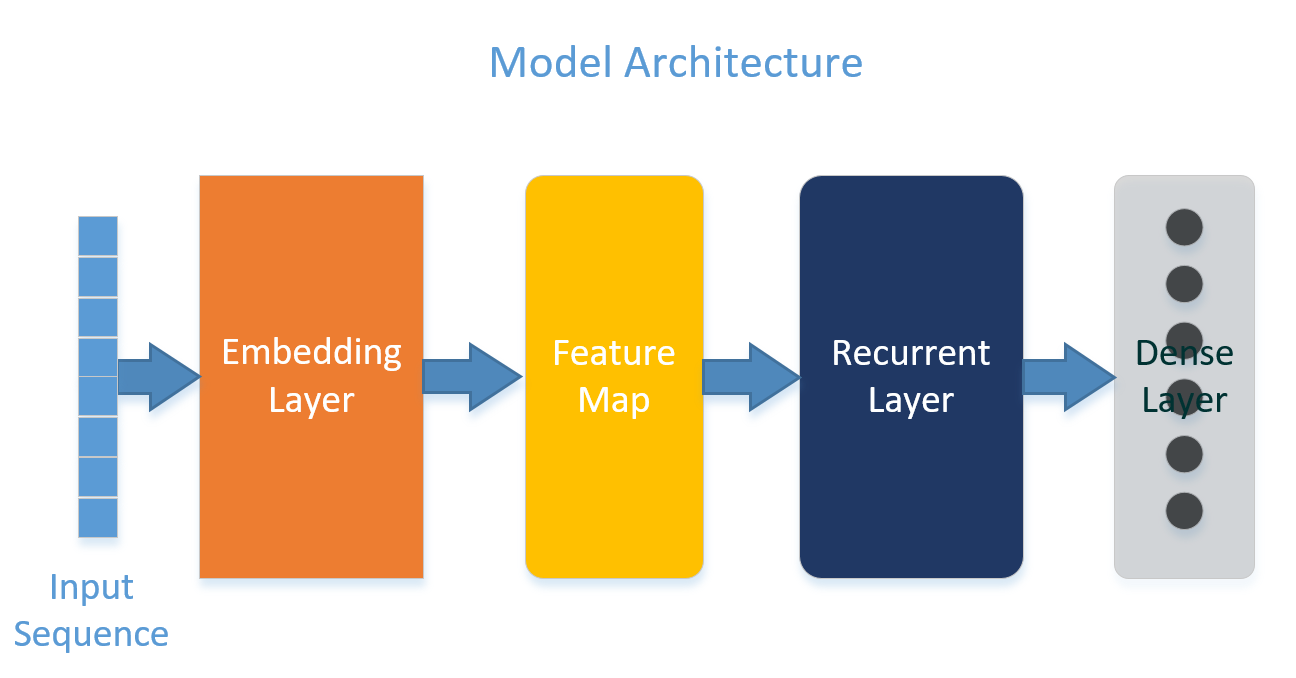
\includegraphics[width=0.5\textwidth]{ModelPipeline.png}
\end{figure}

Our mnetwork model is a variation of the convolutional model proposed by Yoon2014.
Our model consists of an embedding layer, two feature maps, a recurrent layer, and a dense layer.

The network's architecture is as follows:
\begin{itemize}
  \item Input layer: word index vector
  \item Embedding layer: maps word index vector to embedding matrix
  \item Feature Map 1:
      \begin{itemize}
        \item Convolution layer: number of kernels:32, activation: rectified linear
        \item MaxPooling layer
      \end{itemize}
\item Feature Map 2:
    \begin{itemize}
      \item Convolution layer: number of kernels:32, activation: rectified linear
      \item MaxPooling layer
    \end{itemize}
\item Gated Recurrent Unit layer
\item Dropout layer
\item Dense layer: output size: number of classes, activation: softmax
\end{itemize}

\section{Model Hyper-Parameters}
\begin{itemize}
  \item number of training words
  \item number of kernels
  \item kernel size
  \item pool size
  \item learning rate
  \item regularization rate
  \item dropout rate
  \item maximum sequence length

\end{itemize}

\section{Dataset Description}
[DESCRIBE AND CITE EMBEDDINGS]

We gathered scientific paper abstracts from the online repository Arxiv.org.
We scraped papers for 5 departments: computer science, mathematics, astrophysics, physics, quantitative biology, and quantititative finance.

\section{Final Pipeline}
[INCLUDE PIPELINE DIAGRAM]
